%%%%%%%%%%%%%%%%%%%%%%%%%%%%%%% main.tex %%%%%%%%%%%%%%%%%%%%%%%%%%%%%%%
%                                                                      %
% --------------------- Report Template IST [EN] --------------------- %
%                                                                      %
%       João Marafuz Gaspar                                            %
%       Departamento de Engenharia Eletrotécnica e de Computadores     %
%       Instituto Superior Tecnico                                      %
%       Av. Rovisco Pais                                               %
%       1049-001 Lisboa                                                %
%       Portugal                                                       %
%       E-mail: joao.marafuz.gaspar@tecnico.ulisboa.pt                 %
%                                                                      %
%  Created:       Jul 30, 2022                                         %
%  Last Modified: May 18, 2024                                         %
%                                                                      %
%%%%%%%%%%%%%%%%%%%%%%%%%%%%%%%%%%%%%%%%%%%%%%%%%%%%%%%%%%%%%%%%%%%%%%%%
%  Revision history                                                    %
%  v1 - 2022/07/30 - original template                                 %
%  v2 - 2023/04/06 - change superscript in the cover, updated font,    %
%                    added subfigures and table                        %
%  v3 - 18/05/2024 - update for using only one font, known by the name %
%                    of CMU Serif Roman                                %
%%%%%%%%%%%%%%%%%%%%%%%%%%%%%%%%%%%%%%%%%%%%%%%%%%%%%%%%%%%%%%%%%%%%%%%%
%                              Preamble                                %
%%%%%%%%%%%%%%%%%%%%%%%%%%%%%%%%%%%%%%%%%%%%%%%%%%%%%%%%%%%%%%%%%%%%%%%%

% ----------------------------------------------------------------------
% Set the document class
% ----------------------------------------------------------------------
\documentclass[12pt]{article}

% ----------------------------------------------------------------------
% Define external packages, language, margins, fonts, new commands 
% and colors
% ----------------------------------------------------------------------
\usepackage[utf8]{inputenc} % Codification
\usepackage[english]{babel} % Writing idiom

\usepackage[export]{adjustbox} % Align images
\usepackage{amsmath} % Extra commands for math mode
\usepackage{amssymb} % Mathematical symbols
\usepackage{anysize} % Personalize margins
    \marginsize{2cm}{2cm}{2cm}{2cm} % {left}{right}{above}{below}
\usepackage{appendix} % Appendices
\usepackage{cancel} % Expression cancellation
\usepackage{caption} % Captions
    \captionsetup{labelfont={bf}}
\usepackage{cite} % Citations, like [1 - 3]
\usepackage{color} % Text coloring
\usepackage{fancyhdr} % Head note and footnote
    \pagestyle{fancy}
    \fancyhf{}
    \fancyhead[L]{\footnotesize \today} % Left of Head note
    \fancyhead[R]{\footnotesize Piyush Acharya} % Right of Head note
    \fancyfoot[L]{\footnotesize P4 AP/IB Physics 1} % Left of Footnote
    \fancyfoot[C]{\thepage} % Center of Footnote
    \fancyfoot[R]{\footnotesize Momentum Lab} % Right of Footnote
    \renewcommand{\footrulewidth}{0.4pt} % Footnote rule
\usepackage{float} % Utilization of [H] in figures
\usepackage{graphicx} % Figures in LaTeX
\usepackage[colorlinks = true, plainpages = true, linkcolor = istblue, urlcolor = istblue, citecolor = istblue, anchorcolor = istblue]{hyperref}
\usepackage{indentfirst} % First paragraph
\usepackage[super]{nth} % Superscripts
\usepackage{siunitx} % SI units
\usepackage{subcaption} % Subfigures
\usepackage{titlesec} % Font
    \titleformat{\section}{\Large\bfseries}{\thesection}{1em}{}
    \titleformat{\subsection}{\large\bfseries}{\thesubsection}{1em}{}
    \titleformat{\subsubsection}{\normalsize\bfseries}{\thesubsubsection}{1em}{}
\usepackage{pgfplots} % Plotting graphs

% Colors
\definecolor{istblue}{RGB}{3, 171, 230}
\definecolor{dkgreen}{rgb}{0,0.6,0}
\definecolor{gray}{rgb}{0.5,0.5,0.5}

% Random text (not needed)
\usepackage{lipsum}
\usepackage{duckuments}

% New and re-newcommands
\newcommand{\sen}{\operatorname{\sen}} % Sine function definition
\newcommand{\HRule}{\rule{\linewidth}{0.5mm}} % Specific rule definition
\renewcommand{\appendixpagename}{\LARGE Appendices}

%%%%%%%%%%%%%%%%%%%%%%%%%%%%%%%%%%%%%%%%%%%%%%%%%%%%%%%%%%%%%%%%%%%%%%%%
%                                 Document                             %
%%%%%%%%%%%%%%%%%%%%%%%%%%%%%%%%%%%%%%%%%%%%%%%%%%%%%%%%%%%%%%%%%%%%%%%%
\begin{document}

% ----------------------------------------------------------------------
% Cover
% ----------------------------------------------------------------------
\begin{center}
    \begin{figure}
        \vspace{-1.0cm}
        
\includegraphics[scale=0.3, left]{Images/IST_B.png} % IST logo
    \end{figure}
    \mbox{}\\[2.0cm]
    \textsc{\Huge AP/IB Physics 1}\\[2.5cm]
    \textsc{\LARGE Period 4}\\[2.0cm]
    \HRule\\[0.4cm]
    {\large \bf {Momentum Lab}}\\[0.2cm]
    \HRule\\[1.5cm]
\end{center}

\begin{flushleft}
    \textbf{Authors:}
\end{flushleft}

\begin{center}
    \begin{minipage}{0.5\textwidth}
        \begin{flushleft}
            Piyush Acharya\\
        \end{flushleft}
    \end{minipage}%
    \begin{minipage}{0.5\textwidth}
        \begin{flushright}
            \href{mailto:hey@piyushacharya.com}{\texttt{hey@piyushacharya.com}}\\
        \end{flushright}
    \end{minipage}
\end{center}
    
\begin{center}
    \large \bf 2023/2024 -- \nth{2} Semester, P4
\end{center}

\thispagestyle{empty}

\setcounter{page}{0}

\newpage

% ----------------------------------------------------------------------
% Contents
% ----------------------------------------------------------------------
\tableofcontents 

\newpage

% ----------------------------------------------------------------------
% Body
% ----------------------------------------------------------------------
\section{Introduction}

The purpose of this lab is to investigate whether the force between two objects remains the same when they collide with different initial velocities. We conducted five trials, changing the initial velocity of the colliding objects, with one object remaining stationary in each. Video analysis was used to determine the duration of the collision and the change in velocity for the non-stationary object. The change in velocity was measured immediately before and after the collision.

\subsection*{Procedure}

\begin{enumerate}
    \item Set up the track and cart system with the cart at the end of the track.
    \item Place the textbooks at the end of the track and assign 1 person to hold them in place.
    \item Assign another person to release the cart at the start of the track with varying initial velocities.
    \item Record the collision using a video camera.
    \item Analyze the video to determine the time duration of the collision and the change in velocity of the cart.
\end{enumerate}

For each measurement, the following procedures were followed:
\begin{enumerate}
    \item Mass measurement: The mass of the cart was measured using a digital scale with an error estimation of +/- 0.00001 kg.
    
    \item Time duration measurement: The time duration of the collision was determined by analyzing the recorded video. The video analysis software was used to identify the start and end frames of the collision, and the time difference between these frames was calculated. The error estimation for the time duration measurement depends on the frame rate of the video and the accuracy of the video analysis software.
    
    \item Change in velocity measurement: The change in velocity of the cart was also determined by analyzing the recorded video. The initial and final velocities of the cart were measured by tracking its position in the video frames. The change in velocity was then calculated as the difference between the final and initial velocities.
\end{enumerate}

Please note that the specific error estimations for the time duration and change in velocity measurements may vary depending on the equipment and software used in the experiment.

\section{Data Collection}
\begin{table}[H]
    \centering
    \caption{Summary of Experimental Data}
    \label{tab:data}
    \resizebox{\textwidth}{!}{%
    \begin{tabular}{|c|c|c|c|c|c|c|c|}
        \hline
        Trial & Initial Velocity (cart) & Initial Velocity (textbooks) & Final Velocity (cart) & Time (s) & Change in Velocity (m/s) & Error in $\Delta v$ (m/s) & Mass (kg) \\ \hline
        1     & 0.69                   & 0                           & -0.82                 & 0.238    & 1.51      & $\pm 0.05$ & 0.50 \\ \hline
        2     & 0.75                   & 0                           & -0.45                 & 0.292    & 1.20      & $\pm 0.05$ & 0.50 \\ \hline
        3     & 0.66                   & 0                           & -0.51                 & 0.31     & 1.17      & $\pm 0.05$ & 0.50 \\ \hline
        4     & 0.26                   & 0                           & -0.17                 & 0.193    & 0.43      & $\pm 0.05$ & 0.50 \\ \hline
        5     & 0.72                   & 0                           & -0.54                 & 0.25     & 1.26      & $\pm 0.05$ & 0.50 \\ \hline
    \end{tabular}%
    }
\end{table}

\section{Analysis \& Error Treatment}

Using the collected data, we can plot the graph of $m \cdot \Delta v$ vs. $t$ to determine if the force remains constant during the collision. According to the equation $mv = Ft$, the slope of this graph should equal the force.

\begin{figure}[H]
    \centering
    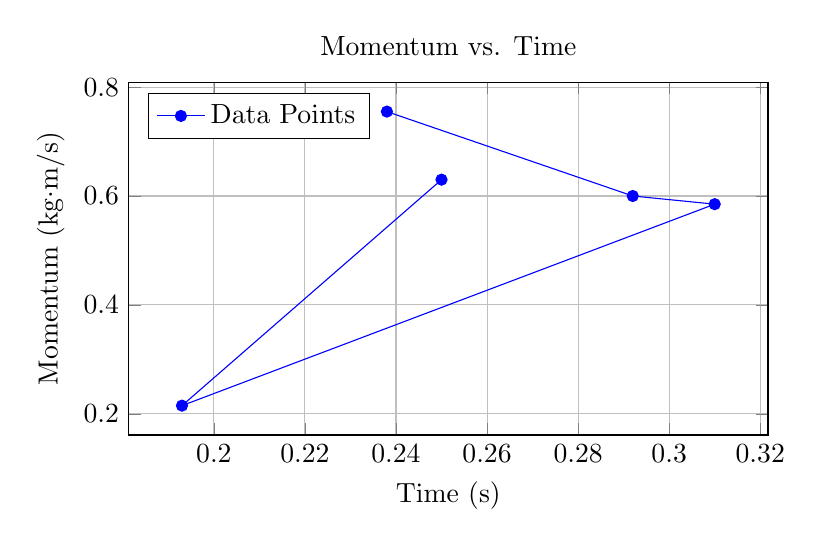
\begin{tikzpicture}
    \begin{axis}[
        title={Momentum vs. Time},
        xlabel={Time (s)},
        ylabel={Momentum (kg$\cdot$m/s)},
        legend pos=north west,
        grid=major,
        width=0.8\textwidth,
        height=0.5\textwidth
    ]
    \addplot[color=blue, mark=*] coordinates {
        (0.238, 0.755)
        (0.292, 0.60)
        (0.31, 0.585)
        (0.193, 0.215)
        (0.25, 0.63)
    };
    \legend{Data Points}
    \end{axis}
    \end{tikzpicture}
    \caption{Graph of $m \cdot \Delta v$ vs. Time}
    \label{fig:momentum_vs_time}
\end{figure}.../.   
\subsection{Error Calculation}
To determine the error in force, we use the formula:
\[
\sigma_F = \left| F \right| \sqrt{\left( \frac{\sigma_m}{m} \right)^2 + \left( \frac{\sigma_{\Delta v}}{\Delta v} \right)^2 + \left( \frac{\sigma_t}{t} \right)^2}
\]
where:
\[
\sigma_m = 0.01 \, \text{kg}, \quad \sigma_{\Delta v} = 0.05 \, \text{m/s}, \quad \sigma_t = 0.01 \, \text{s}
\]

\subsubsection{Example Error Calculation for Trial 1}
\begin{align*}
\sigma_F &= \left| 3.17 \, \text{N} \right| \sqrt{\left( \frac{0.01 \, \text{kg}}{0.50 \, \text{kg}} \right)^2 + \left( \frac{0.05 \, \text{m/s}}{1.51 \, \text{m/s}} \right)^2 + \left( \frac{0.01 \, \text{s}}{0.238 \, \text{s}} \right)^2} \\
&\approx 3.17 \, \text{N} \sqrt{0.0004 + 0.0011 + 0.0018} \\
&\approx 3.17 \, \text{N} \cdot 0.052 \\
&\approx 0.165 \, \text{N}
\end{align*}

\section{Conclusion}
Based on the analysis, we can conclude that the force during the collisions remains approximately constant as indicated by the linear relationship in the graph of $m \cdot \Delta v$ vs. time. The range of force values is determined by the slopes of the trendlines.

\section{References}
\begin{thebibliography}{9}
\bibitem{labguide}
Momentum Lab Guidance Document, AP/IB Physics 1, Melissa Shemwell.
\bibitem{errordoc}
Types of Error Document, AP/IB Physics 1, Melissa Shemwell.
\end{thebibliography}

% ----------------------------------------------------------------------
% Appendices
% ----------------------------------------------------------------------
\appendix  
\clearpage
\addappheadtotoc 
\appendixpage 

\section{Raw Data}
Include any raw data or additional calculations here.

\end{document}
